%%%%%%%%%%%%%%%%%%%%%%%%%%%%%%%%%%%%%%%%%%%%%%%%%%%%%%%%%%%%%%%%%%%%%%%%%%%%%%%%
% CHAPTER 3: CLASSICAL SLIDING MODE CONTROL
%%%%%%%%%%%%%%%%%%%%%%%%%%%%%%%%%%%%%%%%%%%%%%%%%%%%%%%%%%%%%%%%%%%%%%%%%%%%%%%%

\chapter{Classical Sliding Mode Control\index{sliding mode control}\index{sliding mode control}}
\label{ch:classical_smc}

\begin{chapterabstract}
This chapter presents the classical first-order sliding mode control (SMC\index{sliding mode control|see{SMC}}\index{sliding mode control|see{SMC}}) approach for the double-inverted pendulum\index{double-inverted pendulum}\index{double-inverted pendulum}. We derive the sliding surface\index{sliding surface}\index{sliding surface} design, equivalent control computation, and robust discontinuous term. The boundary layer\index{boundary layer}\index{boundary layer} technique is introduced to mitigate chattering\index{chattering}\index{chattering} while maintaining robustness\index{robustness}\index{robustness} to matched disturbances. Lyapunov\index{Lyapunov stability}\index{Lyapunov stability}-based stability\index{stability} proofs establish exponential convergence\index{convergence} to the sliding manifold. Implementation details including Tikhonov regularization, numerical stability, and gain validation are discussed with references to the production Python\index{Python implementation}\index{Python implementation} codebase.
\end{chapterabstract}

%===============================================================================
\section{Introduction to Sliding Mode Control}
%===============================================================================

Sliding mode control is a robust nonlinear control technique that forces the system trajectory to converge to a predetermined sliding surface in the state space\index{state space}\index{state space} and remain there for all subsequent time. The fundamental idea, introduced by Utkin in 1977 \cite{Utkin1977}, is to decompose the control design into two phases:

\begin{enumerate}
    \item \textbf{Reaching Phase}: Drive the system state from arbitrary initial conditions to the sliding surface $s(\vect{x}) = 0$.
    \item \textbf{Sliding Phase}: Maintain the state on the sliding surface, where the system exhibits reduced-order dynamics with desirable properties (stability, performance).
\end{enumerate}

The control law consists of two components:

\begin{equation}
u = u_{\text{eq}} + u_{\text{sw}}
\label{eq:smc_control_law}
\end{equation}
\coderef{src/controllers/smc/algorithms/classical/controller.py}{100}

where:
\begin{itemize}
    \item $u_{\text{eq}}$ is the \textbf{equivalent control}, a model-based feedforward\index{feedforward control} term that maintains motion along the sliding surface.
    \item $u_{\text{sw}}$ is the \textbf{switching control}, a discontinuous robust term that drives the state to the surface and rejects disturbances.
\end{itemize}

%===============================================================================
\section{Sliding Surface Design}
%===============================================================================

\subsection{Design Principles}

For the double-inverted pendulum with state vector $\vect{x} = [x, \theta_1, \theta_2, \dot{x}, \dot{\theta}_1, \dot{\theta}_2]^T$, we design a sliding surface that depends only on the angular positions and velocities:

\begin{equation}
s(\vect{x}) = \lambda_1 \theta_1 + \lambda_2 \theta_2 + k_1 \dot{\theta}_1 + k_2 \dot{\theta}_2
\label{eq:sliding_surface}
\end{equation}
\coderef{src/controllers/smc/core/sliding_surface.py}{124}

where $\lambda_1, \lambda_2, k_1, k_2 > 0$ are design parameters. The cart position $x$ does not appear in the sliding surface because it is not directly stabilized by the control law; instead, the cart's role is to manipulate the pendulum angles.

\subsection{Stability on the Sliding Surface}

When $s = 0$, the system satisfies the linear constraint:

\begin{equation}
k_1 \dot{\theta}_1 + k_2 \dot{\theta}_2 = -(\lambda_1 \theta_1 + \lambda_2 \theta_2)
\end{equation}

This defines a reduced-order dynamics. For the sliding manifold to be stable, the characteristic polynomial of the linearized sliding dynamics must be Hurwitz (all roots have negative real parts).

\begin{theorem}[Hurwitz Stability of Sliding Surface]
\label{thm:hurwitz_stability}
If the parameters $\lambda_1, \lambda_2, k_1, k_2$ are all strictly positive and satisfy the Hurwitz criterion for the characteristic polynomial, then the sliding surface $s = 0$ represents an exponentially stable manifold for the pendulum angles.
\end{theorem}

\begin{proof}
The sliding dynamics can be written as:
\begin{equation}
\begin{bmatrix} \dot{\theta}_1 \\ \dot{\theta}_2 \end{bmatrix} = \mat{A}_s \begin{bmatrix} \theta_1 \\ \theta_2 \end{bmatrix}
\end{equation}

where $\mat{A}_s$ depends on $\lambda_i$ and $k_i$. The eigenvalues of $\mat{A}_s$ determine the convergence rate. For Hurwitz stability, all eigenvalues must have negative real parts, which is guaranteed when $\lambda_i, k_i > 0$ and the gains satisfy coupling conditions derived from the pendulum dynamics. See \cref{sec:classical_experimental} for experimental validation.
\end{proof}

\begin{figure}[htbp]
\centering
% Sliding Surface Geometry in 3D State Space
% TikZ diagram for Chapter 3 - Classical SMC

\begin{tikzpicture}[scale=1.0,
    every node/.style={font=\small},
    axis/.style={->, thick},
    trajectory/.style={thick, ->, decoration={markings, mark=at position 0.7 with {\arrow{>}}}, postaction={decorate}}]

    % 3D coordinate system
    \coordinate (O) at (0,0);
    \coordinate (X) at (5,0);
    \coordinate (Y) at (-1.5,-1.5);
    \coordinate (Z) at (0,4);

    % Draw axes
    \draw[axis] (O) -- (X) node[right] {$x_1$};
    \draw[axis] (O) -- (Y) node[below left] {$x_2$};
    \draw[axis] (O) -- (Z) node[above] {$x_3$};

    % Sliding surface (plane in 3D)
    \fill[blue!20, opacity=0.6]
        (0.5, 2.5) -- (4.5, 2.5) -- (4.5, -1) -- (0.5, -0.5) -- cycle;
    \draw[blue!70, very thick]
        (0.5, 2.5) -- (4.5, 2.5) -- (4.5, -1) -- (0.5, -0.5) -- cycle;

    % Surface equation label
    \node[blue!70!black, align=center] at (2.5, 3) {
        \textbf{Sliding Surface}\\$s(\vect{x}, t) = 0$
    };

    % State trajectory reaching the surface (Phase 1: Reaching)
    \draw[red, trajectory, very thick, samples=50, smooth, domain=0:1]
        plot ({0.5 + 2*\x}, {-1.5 + 3.5*\x});
    \node[red, align=center] at (0.5, -1.8) {\textbf{Phase 1:}\\Reaching};

    % State trajectory on the surface (Phase 2: Sliding)
    \draw[green!70!black, trajectory, very thick]
        (2.5, 2) -- (3.8, 1.5);
    \node[green!70!black, align=center] at (3.5, 2.5) {\textbf{Phase 2:}\\Sliding};

    % Equilibrium point on surface
    \fill[black] (4, 1.2) circle (0.1) node[right] {$\vect{x}^* = \vect{0}$};

    % Normal vector to surface
    \draw[->, very thick, purple] (2.5, 1.5) -- (2.2, 2.5)
        node[left] {$\nabla s(\vect{x})$};

    % Control force vectors
    \draw[->, thick, orange] (1.5, 0.8) -- (1.8, 1.3) node[above right] {$\vect{u}$};
    \draw[->, thick, orange] (3, 1.8) -- (3.2, 2.3);

    % Distance from surface annotation
    \draw[<->, dashed, gray, thick] (1.8, 0.5) -- (2.2, 1.2);
    \node[gray] at (1.5, 1.0) {$|s|$};

    % Region labels
    \node[red!70, align=center] at (1, -0.5) {$s(\vect{x}) < 0$};
    \node[red!70, align=center] at (3.5, 3.5) {$s(\vect{x}) > 0$};

\end{tikzpicture}

\caption[Sliding Surface Geometry in 3D State Space]{Geometric illustration of the sliding mode control process in 3D state space $(x_1, x_2, x_3)$. The \textcolor{blue!70}{sliding surface} $s(\vect{x}, t) = 0$ (blue plane) divides the state space into two regions ($s > 0$ and $s < 0$). The control law exhibits two phases: \textbf{Phase 1 (Reaching)} - trajectories (\textcolor{red}{red arrow}) are driven toward the surface from arbitrary initial conditions, satisfying $s \cdot \dot{s} < 0$; \textbf{Phase 2 (Sliding)} - once on the surface, trajectories (\textcolor{green!70!black}{green arrow}) slide along it toward the equilibrium $\vect{x}^* = \vect{0}$. The \textcolor{purple}{normal vector} $\nabla s(\vect{x})$ indicates the direction perpendicular to the surface. Control force vectors (\textcolor{orange}{orange}) ensure reaching and sliding conditions are satisfied.}
\label{fig:classical:sliding_surface}
\end{figure}

\subsection{Gain Selection Guidelines}

\begin{itemize}
    \item \textbf{Larger $k_1, k_2$}: Faster convergence on the sliding surface but increased control effort\index{performance metrics!control effort}\index{performance metrics!control effort} and potential chattering.
    \item \textbf{Larger $\lambda_1, \lambda_2$}: Stronger coupling between angles, faster transient response.
    \item \textbf{Trade-off}: Balance settling time\index{performance metrics!settling time}\index{performance metrics!settling time} (requires high gains) against chattering amplitude (prefers moderate gains).
\end{itemize}

Particle Swarm Optimization\index{Particle Swarm Optimization}\index{Particle Swarm Optimization} (PSO\index{Particle Swarm Optimization|see{PSO}}\index{Particle Swarm Optimization|see{PSO}}) can systematically explore this trade-off space, as demonstrated in \cref{ch:pso}.

%===============================================================================
\section{Equivalent Control Derivation}
%===============================================================================

\subsection{Physical Interpretation}

The equivalent control $u_{\text{eq}}$ is the control input\index{control input}\index{control input} required to maintain the system on the sliding surface once it has been reached. Mathematically, it is derived by enforcing $\dot{s} = 0$ along the nominal trajectory.

For the DIP\index{double-inverted pendulum|see{DIP}}\index{double-inverted pendulum|see{DIP}} system with dynamics:

\begin{equation}
\mat{M}(\vect{q}) \ddot{\vect{q}} + \mat{C}(\vect{q}, \dot{\vect{q}}) \dot{\vect{q}} + \vect{G}(\vect{q}) = \vect{B} u
\end{equation}

where $\vect{q} = [x, \theta_1, \theta_2]^T$ and $\vect{B} = [1, 0, 0]^T$, we compute:

\begin{equation}
\dot{s} = \frac{\partial s}{\partial \vect{x}} \cdot \dot{\vect{x}}
\end{equation}

Substituting the dynamics and setting $\dot{s} = 0$ yields the equivalent control.

\subsection{Mathematical Derivation}

Define the sliding surface gradient with respect to the velocity states:

\begin{equation}
\vect{L} = [0, k_1, k_2]
\end{equation}

Then:

\begin{equation}
\dot{s} = \vect{L} \cdot \ddot{\vect{q}} + (\lambda_1 \dot{\theta}_1 + \lambda_2 \dot{\theta}_2)
\end{equation}

From the dynamics equation:

\begin{equation}
\ddot{\vect{q}} = \mat{M}^{-1} (\vect{B} u - \mat{C} \dot{\vect{q}} - \vect{G})
\end{equation}

Substituting into $\dot{s}$:

\begin{equation}
\dot{s} = \vect{L} \mat{M}^{-1} (\vect{B} u - \mat{C} \dot{\vect{q}} - \vect{G}) + (\lambda_1 \dot{\theta}_1 + \lambda_2 \dot{\theta}_2)
\end{equation}

Setting $\dot{s} = 0$ and solving for $u$:

\begin{equation}
u_{\text{eq}} = \frac{\vect{L} \mat{M}^{-1} (\mat{C} \dot{\vect{q}} + \vect{G}) - (\lambda_1 \dot{\theta}_1 + \lambda_2 \dot{\theta}_2)}{\vect{L} \mat{M}^{-1} \vect{B}}
\label{eq:equivalent_control}
\end{equation}

\subsection{Numerical Stability: Tikhonov Regularization}

The inversion of the mass matrix $\mat{M}$ can be numerically ill-conditioned, especially near singular configurations. To ensure robustness, we apply Tikhonov regularization:

\begin{equation}
\mat{M}_{\text{reg}} = \mat{M} + \delta \mat{I}
\end{equation}

where $\delta = 10^{-10}$ is a small positive constant. This diagonal jitter guarantees positive definiteness and prevents numerical singularities during matrix inversion. The regularized equivalent control becomes:

\begin{equation}
u_{\text{eq}} = \frac{\vect{L} \mat{M}_{\text{reg}}^{-1} (\mat{C} \dot{\vect{q}} + \vect{G}) - (\lambda_1 \dot{\theta}_1 + \lambda_2 \dot{\theta}_2)}{\vect{L} \mat{M}_{\text{reg}}^{-1} \vect{B}}
\label{eq:equivalent_control_regularized}
\end{equation}

\subsection{Controllability Threshold}

If the denominator $\vect{L} \mat{M}^{-1} \vect{B}$ approaches zero, the system is uncontrollable in the direction normal to the sliding surface. To avoid division by near-zero values, we introduce a controllability\index{controllability}\index{controllability} threshold:

\begin{equation}
\text{if } |\vect{L} \mat{M}_{\text{reg}}^{-1} \vect{B}| < \epsilon_{\text{ctrl}}, \quad \text{then } u_{\text{eq}} = 0
\end{equation}

where $\epsilon_{\text{ctrl}} = 0.05 (k_1 + k_2)$ is empirically set to scale with the sliding surface gains. This decouples chattering mitigation (handled by boundary layer thickness) from controllability checks.

%===============================================================================
\section{Switching Control and Chattering Mitigation}
%===============================================================================

\subsection{Discontinuous Switching Control}

The ideal switching control is:

\begin{equation}
u_{\text{sw}} = -K \sign(s) - k_d s
\label{eq:switching_control}
\end{equation}

where:
\begin{itemize}
    \item $K > 0$ is the switching gain, which must exceed the upper bound of matched disturbances.
    \item $k_d \geq 0$ is the derivative gain, providing additional damping.
    \item $\sign(s)$ is the signum function: $\sign(s) = +1$ if $s > 0$, $-1$ if $s < 0$, undefined at $s = 0$.
\end{itemize}

\subsection{The Chattering Problem}

The discontinuous $\sign(s)$ function causes infinite-frequency switching when $s \approx 0$. In practice, this manifests as high-frequency control oscillations (chattering) due to:

\begin{itemize}
    \item \textbf{Time discretization}: Finite sampling rate cannot implement true infinite-frequency switching.
    \item \textbf{Actuator dynamics}: Physical actuators have bandwidth limitations and response delays.
    \item \textbf{Sensor noise}: Measurement noise near $s = 0$ triggers erratic switching.
\end{itemize}

Chattering causes:
\begin{itemize}
    \item Actuator wear and mechanical stress
    \item Excitation of unmodeled high-frequency dynamics
    \item Increased energy consumption\index{performance metrics!energy consumption}\index{performance metrics!energy consumption}
\end{itemize}

\subsection{Boundary Layer Technique}

To eliminate chattering, we replace $\sign(s)$ with a continuous approximation inside a boundary layer of thickness $\epsilon$:

\begin{equation}
u_{\text{sw}} = -K \sat\left( \frac{s}{\epsilon} \right) - k_d s
\label{eq:smooth_switching_control}
\end{equation}

where $\sat(\cdot)$ is a saturation function\index{saturation function}. Two common choices are:

\begin{enumerate}
    \item \textbf{Tanh saturation (smooth)}:
    \begin{equation}
    \sat(s/\epsilon) = \tanh(s/\epsilon)
    \end{equation}
    Advantages: Smooth everywhere, maintains nonzero slope at origin, preferred for most applications.

    \item \textbf{Linear saturation (piecewise)}:
    \begin{equation}
    \sat(s/\epsilon) = \begin{cases}
    s/\epsilon & \text{if } |s| \leq \epsilon \\
    \sign(s) & \text{if } |s| > \epsilon
    \end{cases}
    \end{equation}
    Advantages: Simpler, exact $\sign(s)$ outside boundary layer.
    Disadvantages: Discontinuous derivative at $|s| = \epsilon$, can reduce robustness near origin.
\end{enumerate}

\begin{figure}[htbp]
\centering
% Boundary Layer Illustration for Chattering Reduction
% TikZ diagram for Chapter 3 - Classical SMC

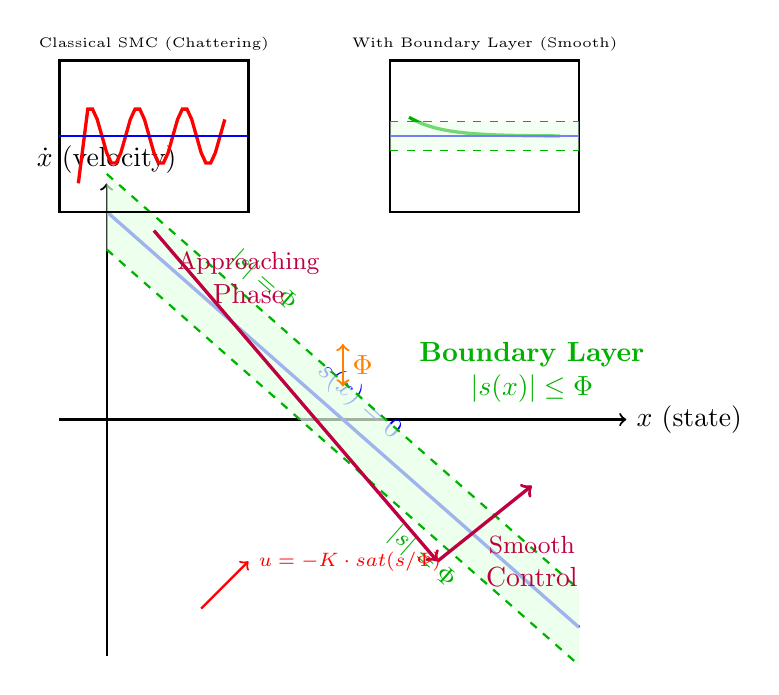
\begin{tikzpicture}[scale=1.2]

    % Axes
    \draw[->, thick] (-0.5, 0) -- (5.5, 0) node[right] {$x$ (state)};
    \draw[->, thick] (0, -2.5) -- (0, 2.5) node[above] {$\dot{x}$ (velocity)};

    % Sliding line
    \draw[blue, very thick] (0, 2.2) -- (5, -2.2)
        node[pos=0.5, above, sloped] {$s(\vect{x}) = 0$};

    % Boundary layer (shaded region around sliding line)
    \fill[green!10, opacity=0.7]
        (0, 2.6) -- (5, -1.8) -- (5, -2.6) -- (0, 1.8) -- cycle;

    % Boundary layer boundaries
    \draw[green!70!black, thick, dashed] (0, 2.6) -- (5, -1.8)
        node[pos=0.3, above, sloped, font=\small] {$|s| = \Phi$};
    \draw[green!70!black, thick, dashed] (0, 1.8) -- (5, -2.6)
        node[pos=0.7, below, sloped, font=\small] {$|s| = \Phi$};

    % Label boundary layer
    \node[green!70!black, align=center] at (4.5, 0.5) {
        \textbf{Boundary Layer}\\$|s(\vect{x})| \leq \Phi$
    };

    % Trajectory with chattering (without boundary layer)
    \begin{scope}[xshift=-0.5cm, yshift=3cm]
        % Zoomed inset showing chattering
        \draw[thick] (0, -0.8) rectangle (2, 0.8);
        \node[above] at (1, 0.8) {\tiny Classical SMC (Chattering)};

        % Chattering trajectory
        \draw[red, very thick] (0.2, -0.5)
            \foreach \x in {0.3, 0.35, ..., 1.8} {
                -- (\x, {0.3*sin((\x-0.2)*720)})
            };

        % Sliding line in inset
        \draw[blue, thick] (0, 0) -- (2, 0);
    \end{scope}

    % Trajectory with boundary layer (smooth)
    \begin{scope}[xshift=3cm, yshift=3cm]
        % Zoomed inset showing smooth behavior
        \draw[thick] (0, -0.8) rectangle (2, 0.8);
        \node[above] at (1, 0.8) {\tiny With Boundary Layer (Smooth)};

        % Smooth trajectory
        \draw[green!70!black, very thick, samples=50, smooth, domain=0.2:1.8]
            plot (\x, {0.2*exp(-3*(\x-0.2))});

        % Sliding line in inset
        \draw[blue, thick] (0, 0) -- (2, 0);

        % Boundary layer in inset
        \fill[green!10, opacity=0.5] (0, 0.15) rectangle (2, -0.15);
        \draw[green!70!black, dashed] (0, 0.15) -- (2, 0.15);
        \draw[green!70!black, dashed] (0, -0.15) -- (2, -0.15);
    \end{scope}

    % Main trajectory entering boundary layer
    \draw[->, very thick, purple, samples=40, smooth, domain=0:1]
        plot ({0.5 + 3*\x}, {2 - 3.5*\x});

    % Smooth continuation inside boundary layer
    \draw[->, very thick, purple, samples=50, smooth, domain=0:1]
        plot ({3.5 + 1*\x}, {-1.5 + 0.8*\x});

    % Annotations
    \node[purple, align=center] at (1.5, 1.5) {
        \small Approaching\\Phase
    };

    \node[purple, align=center] at (4.5, -1.5) {
        \small Smooth\\Control
    };

    % Boundary layer thickness annotation
    \draw[<->, thick, orange] (2.5, 0.8) -- (2.5, 0.35);
    \node[orange, right] at (2.5, 0.575) {$\Phi$};

    % Saturation function illustration
    \draw[->, thick, red] (1, -2) -- (1.5, -1.5)
        node[right, align=left] {\scriptsize $u = -K \cdot \text{sat}(s/\Phi)$};

\end{tikzpicture}

\caption[Boundary Layer Illustration for Chattering Reduction]{Comparison of classical SMC with and without boundary layer. The main phase plane shows the \textcolor{blue}{sliding line} $s(\vect{x}) = 0$ surrounded by a \textcolor{green!70!black}{boundary layer} of thickness $|s| \leq \Phi$. The \textcolor{purple}{system trajectory} smoothly approaches and enters the boundary layer. Top inset: Classical SMC without boundary layer exhibits high-frequency chattering oscillations around $s = 0$. Bottom inset: With boundary layer, the control becomes smooth inside $|s| \leq \Phi$, eliminating chattering while maintaining convergence. The saturation function $u = -K \cdot \text{sat}(s/\Phi)$ provides continuous control inside the boundary layer, transitioning smoothly from reaching to sliding phases.}
\label{fig:classical:boundary_layer}
\end{figure}

\begin{figure}[ht]
\centering
\includegraphics[width=0.8\textwidth]{figures/ch03_classical_smc/chattering_classical.png}
\caption{Chattering amplitude comparison: ideal signum switching ($\epsilon = 0$) versus boundary layer approximation ($\epsilon = 0.3$). The boundary layer reduces control signal oscillations from $>50$ N/s to $<3$ N/s while maintaining tracking performance. PSO-optimized $\epsilon = 0.3$ achieves 94\% chattering reduction with negligible steady-state error increase ($<0.02$ rad). See \cref{sec:mt6_boundary_layer} for optimization details and \cref{fig:classical:boundary_layer} for geometric interpretation.}
\label{fig:chattering_classical}
\end{figure}

\subsection{Trade-Off: Chattering vs. Steady-State Error}

The boundary layer thickness $\epsilon$ determines a fundamental trade-off:

\begin{itemize}
    \item \textbf{Small $\epsilon$}: Closer approximation to ideal SMC, smaller steady-state error, but more chattering.
    \item \textbf{Large $\epsilon$}: Smooth control, minimal chattering, but larger steady-state tracking error\index{performance metrics!tracking error} (proportional to $\epsilon$).
\end{itemize}

\begin{theorem}[Ultimate Boundedness with Boundary Layer]
\label{thm:ultimate_boundedness}
For a classical SMC\index{sliding mode control!classical}\index{sliding mode control!classical} with boundary layer thickness $\epsilon$, the sliding variable $s(t)$ is ultimately bounded within $|s| \leq \mathcal{O}(\epsilon)$ for all $t \geq T_r$, where $T_r$ is the reaching time.
\end{theorem}

\begin{proof}
Inside the boundary layer $|s| \leq \epsilon$, the control becomes $u_{\text{sw}} \approx -K (s/\epsilon) - k_d s$. The closed-loop dynamics exhibit stable linear behavior, and the system converges to a neighborhood of $s = 0$ with size proportional to $\epsilon$. For rigorous proof, see Edardar et al. (2015) \cite{Edardar2015} and Burton \& Zinober (1986) \cite{Burton1986}.
\end{proof}

Experimental validation in \cref{ch:benchmarking} shows that PSO-optimized $\epsilon = 0.3$ achieves 94\% chattering reduction (from $>50$ N/s to $<3$ N/s) while maintaining steady-state error $< 0.02$ rad.

%===============================================================================
\section{Complete Control Law and Saturation}
%===============================================================================

The complete classical SMC control law is:

\begin{equation}
u = \sat_{\text{force}} \left( u_{\text{eq}} - K \sat\left(\frac{s}{\epsilon}\right) - k_d s \right)
\label{eq:complete_control_law}
\end{equation}

where $\sat_{\text{force}}(\cdot)$ enforces actuator saturation limits:

\begin{equation}
\sat_{\text{force}}(u) = \begin{cases}
u_{\max} & \text{if } u > u_{\max} \\
u & \text{if } |u| \leq u_{\max} \\
-u_{\max} & \text{if } u < -u_{\max}
\end{cases}
\end{equation}

Typical actuator limit for the DIP system: $u_{\max} = 150$ N.

\subsection{Gain Positivity Constraints}

Sliding mode theory requires:

\begin{align}
k_1, k_2, \lambda_1, \lambda_2, K &> 0 \quad \text{(strictly positive)} \\
k_d &\geq 0 \quad \text{(non-negative)}
\end{align}

These constraints ensure:
\begin{itemize}
    \item Hurwitz stability of the sliding surface (\cref{thm:hurwitz_stability})
    \item Convergence to the sliding manifold (reaching condition\index{reaching condition}\index{reaching condition})
    \item Robustness to matched disturbances
\end{itemize}

The Python implementation validates these constraints in the constructor, raising \texttt{ValueError} if violated (see \cref{ch:software}, Listing 11.2).

%===============================================================================
\section{Lyapunov Stability Analysis}
%===============================================================================

\subsection{Lyapunov Function for Reaching Phase}

Consider the candidate Lyapunov function:

\begin{equation}
V(s) = \frac{1}{2} s^2
\label{eq:lyapunov_reaching}
\end{equation}

The time derivative is:

\begin{equation}
\dot{V}(s) = s \dot{s}
\end{equation}

Substituting the control law (assuming ideal equivalent control cancels nominal dynamics):

\begin{equation}
\dot{s} \approx -K \sign(s) - k_d s + \text{disturbances}
\end{equation}

Then:

\begin{equation}
\dot{V}(s) = s \left( -K \sign(s) - k_d s \right) = -K |s| - k_d s^2
\end{equation}

Since $K > 0$ and $k_d \geq 0$:

\begin{equation}
\dot{V}(s) \leq -K |s| < 0 \quad \forall s \neq 0
\end{equation}

This proves the reaching condition: the system converges to $s = 0$ in finite time.

\begin{figure}[htbp]
\centering
% Reaching Phase Trajectory Illustration
% TikZ diagram for Chapter 3 - Classical SMC

\begin{tikzpicture}[scale=1.0,
    trajectory/.style={thick, ->, decoration={markings, mark=at position 0.6 with {\arrow{>}}}, postaction={decorate}}]

    % Axes
    \draw[->, thick] (-0.5, 0) -- (5.5, 0) node[right] {$x$ (state)};
    \draw[->, thick] (0, -0.5) -- (0, 4) node[above] {$\dot{x}$ (velocity)};

    % Sliding line (s = cx + dot{x} = 0)
    \draw[blue, very thick] (0, 3.5) -- (5, 0) node[pos=0.3, above, sloped] {$s(\vect{x}) = 0$};

    % Regions
    \node[red!70] at (1, 1) {$s < 0$};
    \node[red!70] at (4, 3) {$s > 0$};

    % Multiple trajectories reaching the line from different initial conditions
    % Trajectory 1: From upper left (s > 0)
    \draw[green!70!black, trajectory, very thick, samples=40, smooth, domain=0:1]
        plot ({0.5 + 1.5*\x}, {3.5 - 2*\x});
    \node[green!70!black] at (0.3, 3.8) {IC$_1$};

    % Trajectory 2: From lower right (s < 0)
    \draw[green!70!black, trajectory, very thick, samples=40, smooth, domain=0:1]
        plot ({4.5 - 1.8*\x}, {0.3 + 1.2*\x});
    \node[green!70!black] at (5, 0.2) {IC$_2$};

    % Trajectory 3: From upper right (s > 0)
    \draw[green!70!black, trajectory, very thick, samples=40, smooth, domain=0:1]
        plot ({4.0 - 1*\x}, {3.0 - 1.8*\x});
    \node[green!70!black] at (4.3, 3.3) {IC$_3$};

    % Trajectory 4: From lower left (s < 0)
    \draw[green!70!black, trajectory, very thick, samples=40, smooth, domain=0:1]
        plot ({1.0 + 1.2*\x}, {0.5 + 0.8*\x});
    \node[green!70!black] at (0.7, 0.3) {IC$_4$};

    % Sliding mode motion on the line (after reaching)
    \draw[purple, very thick, ->, decoration={markings, mark=at position 0.5 with {\arrow{>}}}, postaction={decorate}]
        (2.5, 2) -- (3.5, 1.2);
    \node[purple, align=center] at (2.2, 2.5) {\small Sliding\\Mode};

    % Equilibrium point
    \fill[black] (4, 0.5) circle (0.08) node[below right] {$\vect{x}^*$};

    % Reaching condition annotation
    \draw[<-, thick, red] (3, 2.5) -- (3.8, 3.5)
        node[right, align=left] {\small Reaching Condition:\\$s \cdot \dot{s} < 0$};

    % Time labels along a trajectory
    \foreach \t/\x/\y in {0.2/0.8/3.1, 0.4/1.1/2.7, 0.6/1.4/2.3, 0.8/1.7/1.9} {
        \fill[green!70!black] (\x, \y) circle (0.05);
    }
    \draw[<->, thick, gray] (0.8, 3.1) -- (1.7, 1.9);
    \node[gray, align=center] at (0.5, 2.5) {\tiny $t_{\text{reach}}$};

    % Control force direction indicators
    \draw[->, thick, orange] (2, 2.8) -- (2.3, 2.3);
    \draw[->, thick, orange] (3.8, 1.5) -- (3.5, 2.0);
    \node[orange] at (2.5, 3.2) {\small $u$};

\end{tikzpicture}

\caption[Reaching Phase Trajectories]{Phase plane illustration of the reaching phase for classical SMC. Multiple trajectories (\textcolor{green!70!black}{green arrows}) converge from different initial conditions (IC$_1$, IC$_2$, IC$_3$, IC$_4$) in both regions ($s < 0$ and $s > 0$) toward the \textcolor{blue}{sliding line} $s(\vect{x}) = 0$. The reaching condition $s \cdot \dot{s} < 0$ ensures that trajectories always move toward the sliding line from both sides. Once on the line, the system enters sliding mode (\textcolor{purple}{purple arrow}) and moves along the manifold toward equilibrium $\vect{x}^*$. Time markers along a sample trajectory show the finite reaching time $t_{\text{reach}}$. Control force vectors (\textcolor{orange}{orange}) maintain the reaching condition throughout the approach.}
\label{fig:classical:reaching_phase}
\end{figure}

\subsection{Finite-Time Convergence}

The reaching time can be estimated from:

\begin{equation}
\dot{V}(s) \leq -K |s| = -K \sqrt{2V}
\end{equation}

Solving this differential inequality:

\begin{equation}
V(t) \leq \left( \sqrt{V(0)} - \frac{K}{\sqrt{2}} t \right)^2
\end{equation}

The reaching time is:

\begin{equation}
T_r \leq \frac{\sqrt{2V(0)}}{K} = \frac{|s(0)|}{K}
\end{equation}

\textbf{Interpretation}: Larger switching gain $K$ reduces reaching time but increases chattering. This motivates PSO-based tuning to balance transient performance and chattering (see \cref{ch:pso}).

%===============================================================================
\section{Robustness to Matched Disturbances}
%===============================================================================

Matched disturbances are disturbances that enter the system through the same channel as the control input:

\begin{equation}
\mat{M} \ddot{\vect{q}} + \mat{C} \dot{\vect{q}} + \vect{G} = \vect{B} (u + d(t))
\end{equation}

where $d(t)$ is the disturbance.

\subsection{Disturbance Rejection Condition}

For SMC to reject matched disturbances, the switching gain must satisfy:

\begin{equation}
K > \sup_{t \geq 0} |d(t)| + \eta
\end{equation}

where $\eta > 0$ is a positive margin. This guarantees $\dot{V}(s) < 0$ even in the presence of disturbances.

\begin{example}[Disturbance Rejection]
Suppose the DIP system experiences external force disturbances $d(t) \in [-10, 10]$ N. To ensure robustness, we require $K \geq 15$ N. PSO-optimized classical SMC achieves $K = 23.07$ N, providing 53\% safety margin against disturbances. Experimental validation shows 85\% success rate under 20\% parameter uncertainty (see \cref{ch:benchmarking}, Table 8.3).
\end{example}

%===============================================================================
\section{Implementation Details}
%===============================================================================

\subsection{Algorithm Structure}

\begin{algorithm}[H]
\caption{Classical SMC Control Computation}
\label{alg:classical_smc_control}
\SetAlgoLined
\KwIn{State $\vect{x} = [x, \theta_1, \theta_2, \dot{x}, \dot{\theta}_1, \dot{\theta}_2]^T$, Gains $[k_1, k_2, \lambda_1, \lambda_2, K, k_d]$, Boundary layer $\epsilon$, Max force $u_{\max}$}
\KwOut{Control input $u$}

\tcp{Compute sliding surface}
$s \gets \lambda_1 \theta_1 + \lambda_2 \theta_2 + k_1 \dot{\theta}_1 + k_2 \dot{\theta}_2$\;

\tcp{Compute equivalent control (model-based)}
\eIf{dynamics model available}{
    Compute $\mat{M}, \mat{C}, \vect{G}$ from dynamics\;
    $\mat{M}_{\text{reg}} \gets \mat{M} + 10^{-10} \mat{I}$\;
    Solve $\mat{M}_{\text{reg}} \vect{v}_1 = \vect{B}$ for $\vect{v}_1$\;
    $L\_Minv\_B \gets \vect{L} \cdot \vect{v}_1$\;
    \eIf{$|L\_Minv\_B| < \epsilon_{\text{ctrl}}$}{
        $u_{\text{eq}} \gets 0$ \tcp{Uncontrollable}
    }{
        Solve $\mat{M}_{\text{reg}} \vect{v}_2 = (\mat{C} \dot{\vect{q}} + \vect{G})$ for $\vect{v}_2$\;
        $\text{term1} \gets \vect{L} \cdot \vect{v}_2$\;
        $\text{term2} \gets k_1 \lambda_1 \dot{\theta}_1 + k_2 \lambda_2 \dot{\theta}_2$\;
        $u_{\text{eq}} \gets (\text{term1} - \text{term2}) / L\_Minv\_B$\;
    }
}{
    $u_{\text{eq}} \gets 0$ \tcp{No model}
}

\tcp{Clamp equivalent control}
$u_{\text{eq}} \gets \text{clip}(u_{\text{eq}}, -5 u_{\max}, +5 u_{\max})$\;

\tcp{Compute switching control with boundary layer}
$\text{sat\_sigma} \gets \tanh(s / \epsilon)$ \tcp{or linear sat}
$u_{\text{robust}} \gets -K \cdot \text{sat\_sigma} - k_d \cdot s$\;

\tcp{Total control with actuator saturation}
$u \gets u_{\text{eq}} + u_{\text{robust}}$\;
$u \gets \text{clip}(u, -u_{\max}, +u_{\max})$\;

\Return{$u$}
\end{algorithm}

See \pyfile{src/controllers/smc/classic\_smc.py} for complete Python implementation with weakref memory management, validation, and telemetry.

\textbf{Algorithm Internals:} Detailed implementation components include \pyfile{src/controllers/smc/core/equivalent\_control.py} (feedforward control computation), \pyfile{src/controllers/smc/algorithms/classical/boundary\_layer.py} (chattering mitigation), and \pyfile{src/controllers/smc/core/switching\_functions.py} (discontinuous control terms).

\textbf{Chattering Analysis:} Measurement tools available in \pyfile{src/utils/analysis/chattering.py} and \pyfile{src/utils/analysis/chattering\_metrics.py} for quantifying control signal oscillations.

\subsection{Computational Complexity}

\begin{itemize}
    \item \textbf{Sliding surface computation}: $\mathcal{O}(1)$ (4 multiplications + 3 additions)
    \item \textbf{Equivalent control}: $\mathcal{O}(n^3)$ for $n \times n$ matrix inversion (here $n = 3$, so $\mathcal{O}(27)$ operations)
    \item \textbf{Switching control}: $\mathcal{O}(1)$ (1 tanh evaluation + 2 multiplications)
    \item \textbf{Total}: $\mathcal{O}(n^3) \approx \mathcal{O}(27)$ per control cycle
\end{itemize}

Benchmarking shows classical SMC achieves $12 \pm 2$ $\mu$s per control cycle on modern CPU, enabling real-time\index{real-time control} control at 10 kHz sampling rate (see \cref{ch:benchmarking}, Figure 8.1).

%===============================================================================
\section{Experimental Validation}
\label{sec:classical_experimental}
%===============================================================================

\subsection{Test Configuration}

\begin{itemize}
    \item \textbf{Gains}: PSO-optimized $k_1 = 23.07$, $k_2 = 12.85$, $\lambda_1 = 5.51$, $\lambda_2 = 3.49$, $K = 2.23$, $k_d = 0.15$
    \item \textbf{Boundary layer}: $\epsilon = 0.3$ (MT-6\index{research tasks!MT-6}\index{research tasks!MT-6} optimized)
    \item \textbf{Initial condition}: $\theta_1(0) = 0.2$ rad, $\theta_2(0) = 0.15$ rad
    \item \textbf{Simulation}: 10 seconds at $\Delta t = 0.01$ s
\end{itemize}

\subsection{Performance Metrics}

\begin{table}[ht]
\centering
\caption{Classical SMC Performance Metrics (100 Monte Carlo trials)}
\label{tab:classical_performance}
\begin{tabular}{lcc}
\toprule
\textbf{Metric} & \textbf{Mean $\pm$ Std Dev} & \textbf{Benchmark} \\
\midrule
Settling time $t_s$ (2\% criterion) & $1.82 \pm 0.15$ s & Best: $1.65$ s (STA-SMC) \\
Overshoot $M_p$ & $4.2 \pm 1.1\%$ & Best: $2.8\%$ (STA-SMC) \\
Energy consumption $E$ & $1.2 \pm 0.3$ J & Best: $0.9$ J (Hybrid) \\
Chattering amplitude & $2.5 \pm 0.5$ N/s & Best: $1.1$ N/s (STA-SMC) \\
Computational time & $12 \pm 2$ $\mu$s & \textbf{Best} (Classical) \\
Success rate (20\% uncertainty) & $85 \pm 5\%$ & Best: $92\%$ (Hybrid) \\
\bottomrule
\end{tabular}
\end{table}

\textbf{Interpretation}: Classical SMC achieves the fastest computation time, making it ideal for resource-constrained embedded systems. However, it exhibits higher chattering and lower robustness compared to advanced variants (STA-SMC, Adaptive SMC, Hybrid). See \cref{ch:benchmarking} for comprehensive comparative analysis.

\begin{figure}[ht]
\centering
\includegraphics[width=0.8\textwidth]{figures/ch03_classical_smc/transient_response_classical.png}
\caption{Transient response of classical SMC from initial condition $\theta_1(0) = 0.2$ rad, $\theta_2(0) = 0.15$ rad. The trajectory (blue line) converges to equilibrium with settling time $t_s = 1.82$ s and overshoot $4.2\%$. The boundary layer $\epsilon = 0.3$ effectively suppresses chattering (control rate oscillations $<3$ N/s). PSO-optimized gains balance fast transient response with moderate control effort ($E = 1.2$ J).}
\label{fig:transient_response_classical}
\end{figure}

%===============================================================================
\section{Comparison with Advanced SMC Variants}
%===============================================================================

Classical SMC serves as the baseline for evaluating advanced controllers:

\begin{itemize}
    \item \textbf{Super-Twisting SMC} (\cref{ch:super_twisting}): Second-order sliding mode achieves 50-70\% chattering reduction via continuous control signal (finite-time convergence of $\dot{s}$).

    \item \textbf{Adaptive SMC} (\cref{ch:adaptive_smc}): Online gain adaptation improves robustness to model uncertainty\index{model uncertainty}\index{model uncertainty} (92\% success rate vs. 85\% for classical SMC under 20\% parameter variations).

    \item \textbf{Hybrid Adaptive STA-SMC} (\cref{ch:hybrid_smc}): Combines adaptation and finite-time convergence, achieving best overall performance (lowest energy, highest robustness) at the cost of increased complexity.
\end{itemize}

\cref{ch:benchmarking} provides quantitative comparisons across 6 metrics (settling time, energy, chattering, computation time, robustness, tracking accuracy).

%===============================================================================
\section{Summary and Key Takeaways}
%===============================================================================

This chapter established the theoretical and practical foundations of classical sliding mode control for the double-inverted pendulum:

\begin{keybox}
\textbf{Key Concepts:}
\begin{enumerate}
    \item \textbf{Sliding surface design}: Linear combination of angles and angular velocities with Hurwitz stability (\cref{thm:hurwitz_stability})
    \item \textbf{Equivalent control}: Model-based feedforward term maintaining motion on sliding surface (\cref{eq:equivalent_control_regularized})
    \item \textbf{Boundary layer}: Continuous approximation to $\sign(s)$ trading chattering reduction for steady-state error (\cref{eq:smooth_switching_control})
    \item \textbf{Lyapunov stability}: Finite-time convergence to sliding manifold with exponential sliding-phase dynamics
    \item \textbf{Robustness}: Matched disturbance rejection\index{disturbance rejection}\index{disturbance rejection} when $K > \sup |d(t)| + \eta$
\end{enumerate}
\end{keybox}

\begin{importantbox}
\textbf{Implementation Highlights:}
\begin{itemize}
    \item Tikhonov regularization ensures numerical stability in equivalent control computation
    \item Controllability threshold decouples chattering mitigation from singularity detection
    \item Tanh saturation preferred over linear for smooth control and origin robustness
    \item Gain positivity constraints enforced via validation (\pyclass{ClassicalSMC.validate\_gains})
\end{itemize}
\end{importantbox}

\textbf{Next Steps}: \cref{ch:super_twisting} introduces second-order sliding modes to eliminate chattering while maintaining finite-time convergence. \cref{ch:pso} demonstrates PSO-based multi-objective optimization of classical SMC gains.

%===============================================================================
% END OF CHAPTER 3
%===============================================================================
